% !TeX root = it-governance-risk-compliance.tex
% !TeX encoding = UTF-8
\chapter{Prinsip Tata Kelola TI dan Peran Direksi}

\section*{Tujuan Pembelajaran}
\begin{itemize}
  \item Menerapkan model \textit{Evaluate, Direct, Monitor} dan prinsip ISO/IEC
  38500:2024 untuk menilai praktik tata kelola sebuah organisasi.
  \item Menyusun matriks hak keputusan TI yang memisahkan pihak yang memberi masukan
  dari pihak yang memutuskan.
  \item Mengkritisi pilihan struktur tata kelola, misalnya komite pengarah TI,
  berdasarkan ukuran dan konteks organisasi.
\end{itemize}

\section{Pendahuluan}

Misalkan Medikara menyetujui Rp8 miliar dari anggaran modernisasi Rp10 miliar untuk
memperbarui aplikasi layanan pasien Medikara+. Setelah enam bulan, tim proyek melaporkan
pemasangan sesuai jadwal pada 5 rumah sakit dan 90 persen pekerjaan selesai. Waktu tunggu
pendaftaran baru turun dari 40 menjadi 38 menit, padahal targetnya 25 menit. Direktur
pelayanan belum dapat menjelaskan siapa yang memastikan penurunan itu. Vendor menganggap
pekerjaannya selesai setelah aplikasi diterima. Kepala TI menunjuk jadwal yang terpenuhi.
Semua pihak bekerja, tetapi tidak ada yang memiliki hasilnya. Masalahnya muncul pada
hubungan antara investasi, manfaat, dan kewenangan.

Tata kelola teknologi informasi (TI) memberi tempat bagi pertanyaan yang melampaui
pekerjaan proyek. Bab 1 sudah membedakan tata kelola dari manajemen. Bab ini menjawab
pertanyaan berikutnya: siapa menilai pilihan, siapa memberi arah, siapa memutuskan, dan
bagaimana pihak yang berwenang memantau hasil. Susunan ini harus sesuai dengan bentuk
badan hukum, anggaran dasar, serta delegasi yang berlaku. Hasil kerja bab ini adalah
matriks hak keputusan dan rancangan piagam komite pengarah TI untuk tonggak C1 capstone.

Bab ini memakai empat rujukan utama. ISO/IEC 38500:2024 dari International Organization
for Standardization (ISO) dan International Electrotechnical Commission (IEC) menjelaskan
prinsip dan model \textit{Evaluate, Direct, Monitor} (EDM). Weill dan Ross menyediakan
kerangka hak keputusan. De Haes, Van Grembergen, Joshi, dan Huygh membahas mekanisme tata
kelola. Wu, Straub, dan Liang menguji hubungan tata kelola dengan kinerja. Standar
menjelaskan arah, matriks membantu membagi kewenangan, dan penelitian menguji mekanisme
yang menghubungkan tata kelola dengan hasil
\cite{iso38500-2024,weill2004,dehaes2020,wu2015}.

\IfFileExists{../figures/ch02-diagram-konsep.png}{%

Gambar \ref{fig:ch02-ilustrasi-bab} merangkum hubungan komponen dan konsep utama bab ini.
\begin{figure}[!htb]
  \centering
  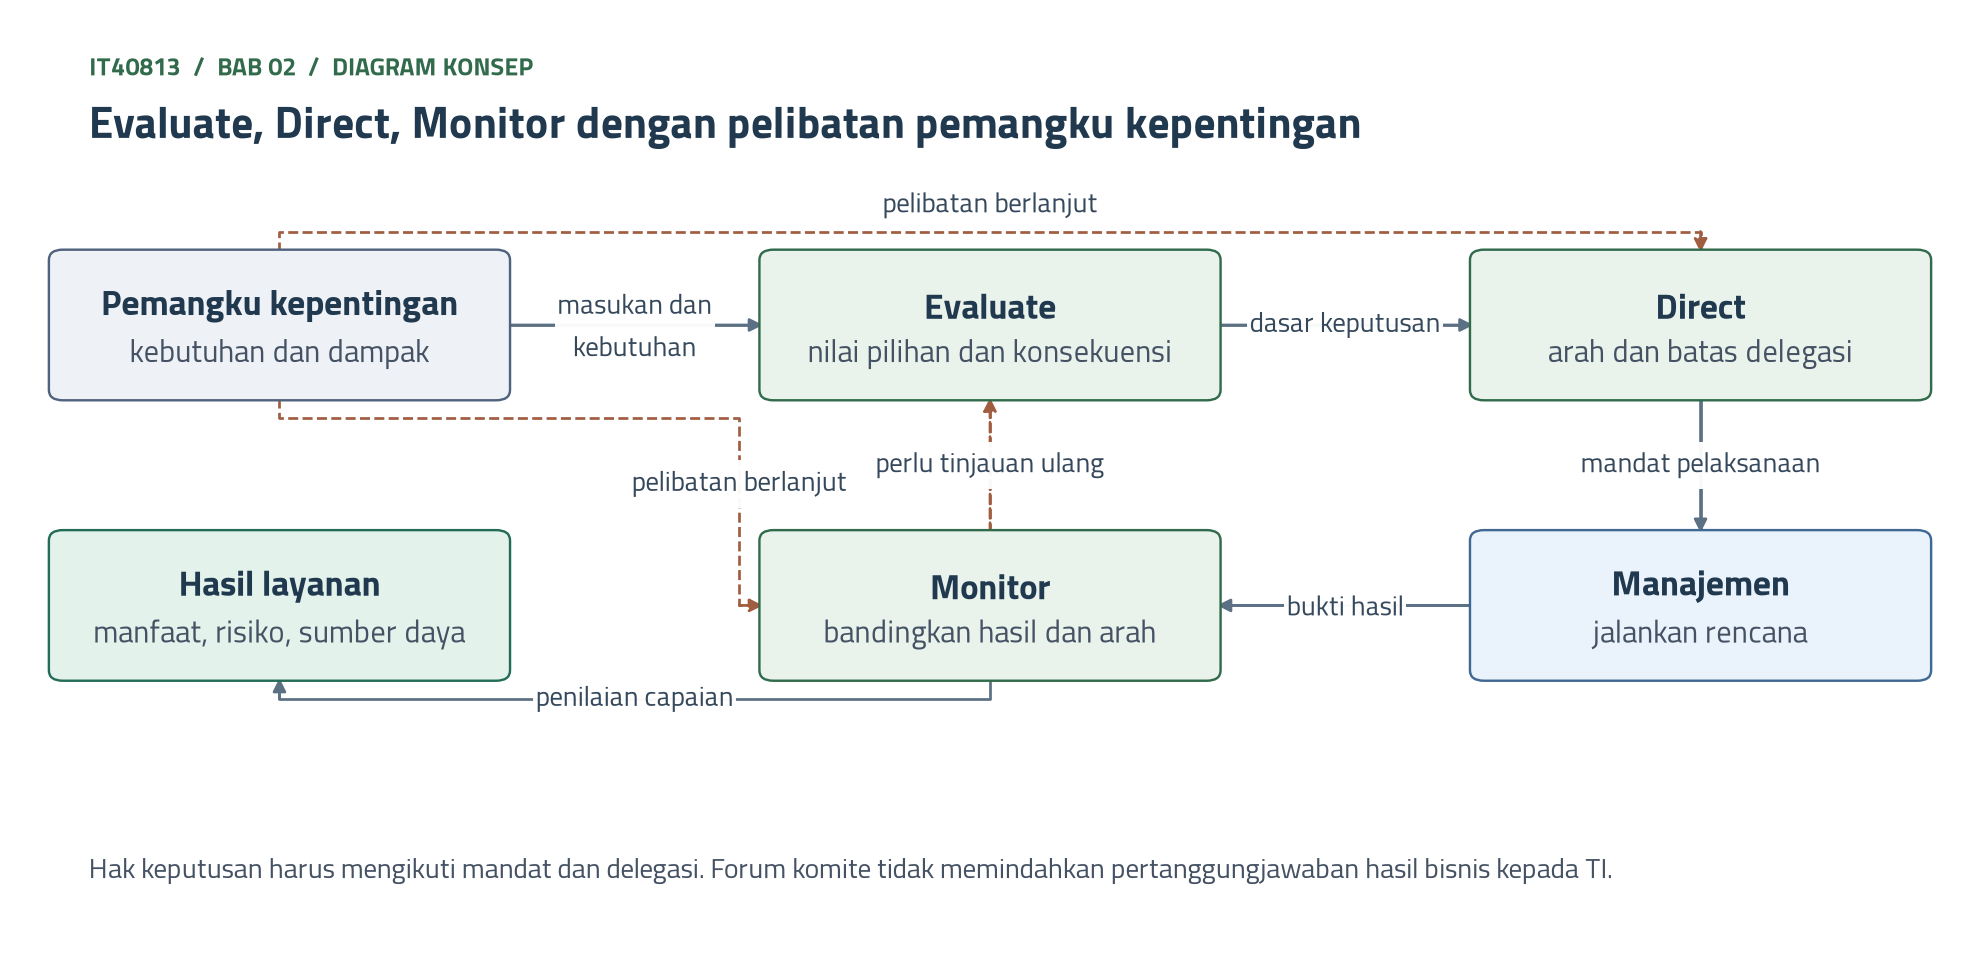
\includegraphics[width=\textwidth]{../figures/ch02-diagram-konsep.png}
  \caption{Evaluate, Direct, Monitor dengan pelibatan pemangku kepentingan}
  \label{fig:ch02-ilustrasi-bab}
\end{figure}
}{}

\section{Tata Kelola Korporat dan Posisi TI}

Pertanyaan pertama: di mana letak TI dalam tata kelola perusahaan? Tata kelola TI bukan
sistem yang berdiri sendiri. \textit{White paper} di situs komite ISO menyebutnya bagian yang
menyatu dengan tata kelola organisasi \cite{c02-iso-perubahan}. Karena itu, penelusuran
kewenangan dimulai dari organ perseroan, bukan dari struktur unit TI.

Pada perseroan terbatas Indonesia, direksi menjalankan pengurusan untuk kepentingan
perseroan, sesuai kebijakan yang dipandang tepat dalam batas undang-undang dan anggaran
dasar. Dewan komisaris mengawasi kebijakan dan jalannya pengurusan, lalu memberi nasihat
kepada direksi. Pembagian tugas antaranggota direksi ditetapkan rapat umum pemegang saham,
atau oleh direksi sendiri bila rapat umum tidak menetapkannya. Pembagian ini perlu dibaca
bersama anggaran dasar dan perubahan peraturan yang berlaku. Pasal 92 dan Pasal 108
Undang-Undang (UU) 40/2007 menjadi titik awal penelusuran, bukan alasan menyalin struktur
perusahaan lain \cite{c02-uu40}.

Organisasi tidak dapat memindahkan seluruh pertanggungjawaban pemanfaatan TI kepada kepala
TI atau vendor. Direktur pelayanan memiliki manfaat layanan. Direktur keuangan memiliki
pertimbangan pendanaan. Fungsi teknologi menjelaskan kelayakan. Komite memberi forum
koordinasi, sedangkan kewenangan hukum tetap mengikuti mandat.
Gambar~\ref{fig:ch02-organ-perseroan} memperlihatkan hubungan itu pada Medikara. Rincian di
bawah direksi adalah pengandaian, karena fakta dasar kasus tidak menyebut susunan
jabatannya.

\begin{figure}[!htb]
  \centering
  \begin{tikzpicture}[
  kotak/.style={draw, rounded corners, align=center, text width=2.85cm,
    minimum height=1.15cm, font=\scriptsize, fill=blue!8},
  panah/.style={-{Stealth[length=2mm]}, thick},
  keterangan/.style={font=\tiny, align=center, inner sep=1pt}
]
  \node[kotak, fill=praditagreen!15] (komisaris) at (0, 4.5)
    {\textbf{Dewan Komisaris}\\{\tiny\mdseries mengawasi dan\\memberi nasihat}};
  \node[kotak, fill=praditagreen!15] (direksi) at (4.45, 4.5)
    {\textbf{Direksi}\\{\tiny\mdseries mengurus perseroan\\dan menetapkan delegasi}};
  \node[kotak, fill=orange!12] (komite) at (8.9, 4.5)
    {\textbf{Komite pengarah TI}\\{\tiny\mdseries forum bermandat,\\bukan organ perseroan}};
  \node[kotak] (pemilik) at (2.225, 2.25)
    {\textbf{Pemilik layanan}\\{\tiny\mdseries direktur pelayanan:\\manfaat dan risiko}};
  \node[kotak] (manajemen) at (6.675, 2.25)
    {\textbf{Manajemen TI}\\{\tiny\mdseries kepala TI:\\kesiapan dan operasi}};
  \node[kotak, fill=green!10] (hasil) at (2.225, 0)
    {\textbf{Hasil layanan}\\{\tiny\mdseries waktu tunggu,\\mutu, dan biaya}};
  \node[kotak] (vendor) at (6.675, 0)
    {\textbf{Vendor}\\{\tiny\mdseries menjalankan pekerjaan\\sesuai kontrak}};
  \draw[panah] ([yshift=2mm]komisaris.east) -- node[keterangan, above]
    {pengawasan\\nasihat} ([yshift=2mm]direksi.west);
  \draw[panah] ([yshift=-2mm]direksi.west) -- node[keterangan, below]
    {laporan} ([yshift=-2mm]komisaris.east);
  \draw[panah] ([yshift=2mm]direksi.east) -- node[keterangan, above]
    {mandat} ([yshift=2mm]komite.west);
  \draw[panah] ([yshift=-2mm]komite.west) -- node[keterangan, below]
    {rekomendasi} ([yshift=-2mm]direksi.east);
  \draw[panah] (direksi.south) -- node[keterangan, fill=white] {delegasi}
    (pemilik.north);
  \draw[panah] (direksi.south) -- node[keterangan, fill=white] {delegasi}
    (manajemen.north);
  \draw[{Stealth[length=2mm]}-{Stealth[length=2mm]}, thick] (pemilik) --
    node[keterangan, above] {kebutuhan\\kesiapan} (manajemen);
  \draw[panah] (pemilik) -- node[keterangan, right] {memiliki\\manfaat} (hasil);
  \draw[panah] (manajemen) -- node[keterangan, right] {mengelola\\kontrak} (vendor);
  \draw[panah] (vendor) -- node[keterangan, above] {pekerjaan} (hasil);
\end{tikzpicture}

  \caption{Organ perseroan, forum komite, dan pemilik hasil pada pengandaian Medikara}
  \label{fig:ch02-organ-perseroan}
\end{figure}

Pengelola rumah sakit dapat meminta penasihat menilai mutu bangunan. Penasihat membantu
menimbang pilihan, tetapi tanda tangan kontrak dan tanggung jawab pengelolaan tetap
mengikuti kewenangan organisasi. Membentuk forum tambahan tidak otomatis memindahkan
tanggung jawab.

Dua contoh penerapannya:
\begin{enumerate}
  \item Misalkan anggaran dasar Medikara mewajibkan persetujuan dewan komisaris untuk
  pengadaan di atas Rp5 miliar. Pasal 117 memberi ruang bagi pengaturan seperti itu.
  Investasi Rp8 miliar melewati batas tersebut. Dewan komisaris kemudian meminta laporan
  risiko modernisasi lima rumah sakit setiap triwulan, atau 4 kali setahun. Direksi tetap
  mengurus program dan menindaklanjuti temuan yang masuk kewenangannya.
  \item Misalkan direktur pelayanan menjadi pemilik manfaat investasi Rp8 miliar. Waktu
  tunggu dipengaruhi jadwal sekitar 640 dokter dan alur kerja di 5 rumah sakit. Kepala TI
  memimpin 52 staf TI dan mengelola kesiapan teknis, tetapi tidak berwenang mengubah jadwal
  dokter. Kepala TI juga tidak sendirian menerima risiko perubahan alur klinis.
\end{enumerate}

Tabel~\ref{tab:ch02-korporat} merangkum peran korporat dan pemanfaatan TI.
\begin{table}[!htb]
  \centering\small
  \caption{Peran korporat dan pemanfaatan TI}\label{tab:ch02-korporat}
  \begin{tabularx}{\textwidth}{|>{\raggedright\arraybackslash}p{0.22\textwidth}|>{\raggedright\arraybackslash}X|>{\raggedright\arraybackslash}X|}
    \hline
    \textbf{Peran} & \textbf{Tanggung jawab contoh} & \textbf{Bukti yang dicari} \\ \hline
    Dewan komisaris & Pengawasan dan nasihat & Notulen pengawasan \\ \hline
    Direksi & Arah, investasi, dan pengurusan & Keputusan serta delegasi \\ \hline
    Pemilik layanan & Hasil dan risiko layanan & Ukuran manfaat \\ \hline
    Manajemen TI & Pelaksanaan serta operasi & Rencana dan laporan kontrol \\ \hline
    Vendor & Pekerjaan sesuai kontrak & Berita acara dan laporan layanan \\ \hline
  \end{tabularx}
\end{table}

\subsection*{Pengurusan dan pengawasan}

Dua hal sering tertukar: pengurusan dan pengawasan. Pembagiannya begini. Pengurusan memilih
tindakan dan menjalankannya. Pengawasan memeriksa kebijakan dan jalannya pengurusan, lalu
memberi nasihat. Komisaris yang memilih vendor Medikara+ sedang masuk ke wilayah pengurusan.
Pasal 118 hanya membuka jalan itu berdasarkan anggaran dasar atau keputusan rapat umum
pemegang saham, untuk keadaan dan jangka waktu tertentu \cite{c02-uu40}.

Pembagian ini menimbulkan kesulitan istilah. Standar internasional memakai kata badan
pengarah (\textit{governing body}) atau \textit{board}. The Institute of Internal Auditors
(IIA) memakai \textit{board} untuk berbagai bentuk badan pengarah beserta komitenya
\cite{iia-tlm2026}. Perseroan Indonesia memisahkan dua organ, sehingga istilah itu tidak
dapat diterjemahkan satu lawan satu. Tabel~\ref{tab:ch02-pemetaan} memberi pemetaan kerja
untuk bab ini. Pemetaan itu penafsiran bab ini, bukan isi standar. Tim tetap perlu
mencocokkannya dengan anggaran dasar organisasi.

\begin{table}[!htb]
  \centering\small
  \caption{Pemetaan kerja tugas tata kelola pada dua organ perseroan}
  \label{tab:ch02-pemetaan}
  \begin{tabularx}{\textwidth}{|>{\raggedright\arraybackslash}p{0.2\textwidth}|>{\raggedright\arraybackslash}X|>{\raggedright\arraybackslash}X|}
    \hline
    \textbf{Tugas} & \textbf{Direksi} & \textbf{Dewan komisaris} \\ \hline
    \textit{Evaluate} & Menilai opsi investasi dan dampaknya & Memberi nasihat; menyetujui
    bila anggaran dasar menetapkan \\ \hline
    \textit{Direct} & Menetapkan arah, pemilik manfaat, dan batas delegasi & Tidak memberi
    perintah operasional \\ \hline
    \textit{Monitor} & Memantau hasil dan memerintahkan koreksi & Mengawasi kebijakan dan
    jalannya pengurusan \\ \hline
    Pelibatan & Mengatur saluran masukan pasien, klinisi, dan unit lokal & Menanyakan
    apakah pihak terdampak sudah didengar \\ \hline
  \end{tabularx}
\end{table}

\subsection*{Akuntabilitas tidak ikut berpindah}

Bila pekerjaan didelegasikan atau dialihkan ke vendor, apakah tanggung jawabnya ikut
berpindah? Tidak seluruhnya. Direksi bertanggung jawab atas pengurusan, dan dewan komisaris
bertanggung jawab atas pengawasan. Anggota kedua organ dapat bertanggung jawab secara
pribadi atas kerugian perseroan bila bersalah atau lalai. Pasal 97 ayat (5) menyebut syarat
pembebasan bagi anggota direksi, antara lain itikad baik, kehati-hatian, dan tidak adanya
benturan kepentingan \cite{c02-uu40}. IIA menyatakan alih daya tidak mengubah akuntabilitas
\textit{board} untuk memastikan kegiatan yang dialihkan berjalan efektif
\cite{iia-tlm2026}. Pernyataan IIA itu membahas kegiatan asurans dan nasihat. Bab ini
memakai logika yang serupa untuk pekerjaan vendor.

Keadaan ini punya dua konsekuensi. Pertama, catatan keputusan bernilai sebagai
pertanggungjawaban. Notulen yang memuat opsi, alasan, dan deklarasi kepentingan membantu
menunjukkan kehati-hatian, meskipun tidak menjamin pembebasan tanggung jawab. Bagian ini
bukan nasihat hukum. Kedua, kontrak menetapkan tugas vendor, tetapi tidak menghapus
kewajiban organisasi menetapkan siapa memantau hasil. Data latihan Bab 1 memperlihatkan
akibatnya: kontrak selesai, akun dukungan tetap aktif, dan 1.240 rekam kunjungan terbaca
selama 8 malam.

\begin{kasus}[title={Kasus Medikara Health: Pertanyaan Komisaris pada Laporan Triwulan}]
Misalkan laporan triwulan menyebut pemasangan Medikara+ sudah mencapai 90 persen. Dewan
komisaris mengajukan tiga pertanyaan. Siapa pemilik manfaat? Berapa selisih hasil terhadap
target? Apa keputusan yang menunggu direksi? Jawaban pertama ternyata berbeda antara
direktur pelayanan dan kepala TI. Jawaban kedua baru tersedia setelah data 5 rumah sakit
dikumpulkan: 38 menit, dari target 25 menit. Jawaban ketiga belum ada.

Dewan komisaris tidak memilih perbaikan, karena memilih perbaikan termasuk pengurusan.
Dewan komisaris menasihati direksi agar menetapkan satu pemilik manfaat dan membawa pilihan
koreksi pada triwulan berikutnya. Direksi lalu menunjuk direktur pelayanan sebagai pemilik
manfaat, sesuai pembagian tugas yang berlaku.
\end{kasus}

\section{ISO/IEC 38500:2024 dan Model Evaluate, Direct, Monitor}

Setelah organnya jelas, apa yang seharusnya dikerjakan? ISO/IEC 38500:2024 memberi panduan
bagi badan pengarah tentang penggunaan TI dalam organisasi \cite{iso38500-2024}. Teks
standar ini berbayar, sehingga rincian berikut mengikuti \textit{white paper} perbedaan
edisi yang terbit di situs komite penyusunnya. Halaman itu memuat penafian bahwa isinya
dikelola pihak ketiga, sehingga tim yang memakainya untuk penilaian formal tetap perlu
memeriksa teks standar \cite{c02-iso-perubahan}.

Edisi 2024 selaras dengan ISO 37000 tentang tata kelola organisasi. Prinsipnya berubah dari
enam menjadi sebelas. Modelnya menambahkan pelibatan pemangku kepentingan
(\textit{engage stakeholders}) di samping tiga tugas EDM. Fokusnya juga bergeser. Tata
kelola tidak lagi dibahas terutama sebagai kerja badan pengarah, tetapi sebagai sesuatu yang
dijalankan di seluruh organisasi, dengan manajemen bekerja dalam kerangka yang ditetapkan
badan pengarah \cite{c02-iso-perubahan}. Tabel~\ref{tab:ch02-edisi} merangkum perbedaannya.

\begin{table}[!htb]
  \centering\small
  \caption{Perbedaan ISO/IEC 38500 edisi 2015 dan edisi 2024}\label{tab:ch02-edisi}
  \begin{tabularx}{\textwidth}{|>{\raggedright\arraybackslash}p{0.18\textwidth}|>{\raggedright\arraybackslash}X|>{\raggedright\arraybackslash}X|}
    \hline
    \textbf{Aspek} & \textbf{Edisi 2015} & \textbf{Edisi 2024} \\ \hline
    Prinsip & Enam: tanggung jawab, strategi, akuisisi, kinerja, kesesuaian, perilaku
    manusia & Sebelas, mengikuti prinsip ISO 37000 \\ \hline
    Model & \textit{Evaluate}, \textit{Direct}, dan \textit{Monitor} oleh badan pengarah &
    Ditambah pelibatan pemangku kepentingan, di atas manajemen TI \\ \hline
    Letak tata kelola & Terutama pada badan pengarah & Di seluruh organisasi, dalam kerangka
    dari badan pengarah \\ \hline
    Kerangka & Konsepnya pertama muncul pada ISO/IEC 38502 & Enam unsur: arah, kapabilitas,
    kebijakan, delegasi, kinerja, akuntabilitas \\ \hline
  \end{tabularx}
\end{table}

Banyak materi daring masih memakai enam prinsip edisi 2015. Daftar itu tidak boleh diberi
label edisi 2024. Tabel~\ref{tab:ch02-prinsip} memuat sebelas prinsip edisi 2024, dengan
kelompok \textit{primary} (utama), \textit{foundational} (dasar), dan \textit{enabling}
(pemungkin). Kolom pertanyaan adalah penerapan bab ini berupa pertanyaan keputusan, bukan
kutipan persyaratan standar.

\begin{table}[!htb]
  \centering\small
  \caption{Sebelas prinsip ISO/IEC 38500:2024 dan pertanyaan penerapannya}
  \label{tab:ch02-prinsip}
  \begin{tabularx}{\textwidth}{|>{\raggedright\arraybackslash}p{0.16\textwidth}|>{\raggedright\arraybackslash}p{0.27\textwidth}|>{\raggedright\arraybackslash}X|}
    \hline
    \textbf{Kelompok} & \textbf{Prinsip} & \textbf{Pertanyaan bagi TI Medikara} \\ \hline
    Utama & Tujuan & Layanan pasien mana yang dilayani TI? \\ \hline
    Dasar & Pembentukan nilai & Nilai apa yang dihasilkan Medikara+? \\ \hline
    Dasar & Strategi & Apakah investasi mendukung ``Satu Pasien, Satu Rekam Medis''? \\
    \hline
    Dasar & Pengawasan & Siapa memeriksa jalannya program? \\ \hline
    Dasar & Akuntabilitas & Siapa menjawab bila target tidak tercapai? \\ \hline
    Pemungkin & Pelibatan pemangku kepentingan & Apakah pasien dan klinisi sudah didengar?
    \\ \hline
    Pemungkin & Kepemimpinan & Siapa memberi contoh dalam memakai data dan aturan? \\
    \hline
    Pemungkin & Data dan keputusan & Apakah keputusan memakai data yang dapat diperiksa? \\
    \hline
    Pemungkin & Tata kelola risiko & Risiko mana yang diterima, dan oleh siapa? \\ \hline
    Pemungkin & Tanggung jawab sosial & Siapa terdampak di luar organisasi? \\ \hline
    Pemungkin & Kelangsungan dan kinerja dari waktu ke waktu & Apakah layanan tetap bertahan
    setelah proyek selesai? \\ \hline
  \end{tabularx}
\end{table}

Prinsip tidak berjalan tanpa kerangka. \textit{White paper} yang sama menyebut enam unsur
kerangka tata kelola menurut edisi 2024 \cite{c02-iso-perubahan}. Keenam unsur itu menjadi
daftar periksa yang berguna saat menilai sebuah organisasi.
Tabel~\ref{tab:ch02-kerangka} menerapkannya pada pengandaian Medikara.

\begin{table}[!htb]
  \centering\small
  \caption{Enam unsur kerangka tata kelola pada pengandaian Medikara}
  \label{tab:ch02-kerangka}
  \begin{tabularx}{\textwidth}{|>{\raggedright\arraybackslash}p{0.2\textwidth}|>{\raggedright\arraybackslash}X|}
    \hline
    \textbf{Unsur} & \textbf{Bentuk pada Medikara} \\ \hline
    Arah & Strategi ``Satu Pasien, Satu Rekam Medis'' 2026 sampai 2030 \\ \hline
    Kapabilitas & 52 staf TI dengan tim platform 6 orang, ditambah vendor Medikara+ \\
    \hline
    Kebijakan & Aturan akses vendor dan standar integrasi \\ \hline
    Delegasi & Batas biaya dan toleransi 10 persen, dijelaskan pada seksi berikutnya \\
    \hline
    Kinerja & Waktu tunggu pendaftaran dari 40 menjadi 25 menit \\ \hline
    Akuntabilitas & Direktur pelayanan sebagai pemilik manfaat, dengan catatan keputusan \\
    \hline
  \end{tabularx}
\end{table}

Evaluasi memerlukan alternatif nyata, termasuk menunda atau menghentikan. Arahan menyebut
batas biaya, pemilik manfaat, risiko yang diterima, dan kondisi penghentian. Pemantauan
membandingkan hasil terhadap arahan dan dapat memicu evaluasi ulang. Pertanyaan kemudian
muncul: siapa perlu dilibatkan? Pihak yang memakai layanan dan menanggung akibat harus
memiliki saluran masukan. Gambar~\ref{fig:ch02-alur} memperlihatkan siklus itu dengan angka
pengandaian Medikara.

\begin{figure}[!htb]
  \centering
  \begin{tikzpicture}[
  kotak/.style={draw, rounded corners, align=center, text width=2.85cm,
    minimum height=1.25cm, font=\scriptsize, fill=blue!8},
  panah/.style={-{Stealth[length=2mm]}, thick},
  keterangan/.style={font=\tiny, align=center, inner sep=1pt}
]
  \node[kotak, fill=praditagreen!15] (pemangku) at (0, 2.6)
    {\textbf{Pemangku}\\\textbf{kepentingan}\\{\tiny\mdseries kebutuhan dan
    dampak:\\pasien, klinisi, unit lokal}};
  \node[kotak] (evaluate) at (4.4, 2.6)
    {\textbf{\textit{Evaluate}}\\{\tiny\mdseries nilai pilihan dan konsekuensi:\\Rp8
    miliar atau Rp6 miliar}};
  \node[kotak] (direct) at (8.8, 2.6)
    {\textbf{\textit{Direct}}\\{\tiny\mdseries arah dan batas delegasi:\\batas Rp8,8
    miliar,\\target 25 menit}};
  \node[kotak] (manajemen) at (8.8, 0)
    {\textbf{Manajemen}\\{\tiny\mdseries jalankan rencana:\\pemasangan di 5 rumah
    sakit}};
  \node[kotak, fill=orange!12] (monitor) at (4.4, 0)
    {\textbf{\textit{Monitor}}\\{\tiny\mdseries bandingkan hasil dan arah:\\38 menit,
    target 25 menit}};
  \node[kotak, fill=green!10] (hasil) at (0, 0)
    {\textbf{Hasil layanan}\\{\tiny\mdseries manfaat, risiko, sumber daya:\\baru 13,3
    persen target}};
  \draw[panah] (pemangku) -- node[keterangan, above]
    {masukan\\dan\\kebutuhan} (evaluate);
  \draw[panah] (evaluate) -- node[keterangan, above]
    {dasar\\keputusan} (direct);
  \draw[panah] (direct) -- node[keterangan, right]
    {mandat\\pelaksanaan} (manajemen);
  \draw[panah] (manajemen) -- node[keterangan, above]
    {bukti\\hasil} (monitor);
  \draw[panah] (monitor) -- node[keterangan, above]
    {penilaian\\capaian} (hasil);
  \draw[panah, dashed] (monitor) -- node[keterangan, right]
    {perlu\\tinjauan\\ulang} (evaluate);
  \draw[panah, densely dotted] (pemangku.south east) -- (monitor.north west);
  \draw[panah, densely dotted] (pemangku.north) -- ++(0, 0.42) -|
    node[keterangan, above, pos=0.25] {pelibatan berlanjut pada ketiga tugas}
    (direct.north);
\end{tikzpicture}

  \caption{Siklus EDM dengan pelibatan pemangku kepentingan pada keputusan Medikara+}
  \label{fig:ch02-alur}
\end{figure}

Panitia renovasi sekolah membandingkan pilihan sebelum memilih kontraktor, menetapkan batas
anggaran dan keselamatan, lalu memeriksa penggunaan ruangan setelah selesai. Guru serta
murid memberi masukan karena mereka mengalami akibat keputusan setiap hari.

Dua contoh penerapannya:
\begin{enumerate}
  \item Misalkan dua opsi aplikasi pasien berbiaya Rp8 miliar dan Rp6 miliar, dengan masa
  pakai 5 tahun. Biaya per tahunnya Rp1,6 miliar dan Rp1,2 miliar. Dengan 336.000 janji
  temu per tahun, biaya per janji temu sekitar Rp4.760 dan Rp3.570. Misalkan opsi pertama
  menargetkan penurunan 15 menit, dan opsi kedua 10 menit. Penghematannya 84.000 jam dan
  56.000 jam per tahun, atau sekitar Rp19.000 dan Rp21.400 per jam. Evaluasi juga menilai
  keselamatan serta kemampuan adopsi, bukan memilih angka terendah secara otomatis.
  \item Misalkan target waktu tunggu turun dari 40 menjadi 25 menit, dengan batas biaya
  Rp8,8 miliar berdasarkan toleransi 10 persen seperti pada Bab 1. Hasil tiga bulan masih
  38 menit, atau baru 2 dari 15 menit yang ditargetkan (13,3 persen). Pemantauan memicu
  peninjauan proses, alokasi petugas, dan rancangan aplikasi. Bila biaya naik 27 persen,
  sesuai rata-rata pada Bab 1, nilainya Rp10,16 miliar dan keputusan kembali ke direksi.
\end{enumerate}

\subsection*{Dua pemantauan yang sering tertukar}

Dua hal pada EDM sering tertukar: \textit{Monitor} sebagai tugas tata kelola dan pemantauan
harian oleh manajemen. Pembagiannya begini. Manajemen memantau jalannya pekerjaan agar
rencana terlaksana. Badan pengarah memantau apakah arah masih benar dan hasilnya sesuai.
Control Objectives for Information and Related Technologies (COBIT) juga memisahkan
keduanya \cite{cobit2019-intro}, dan Bab 4 membahas rinciannya.

Misalkan tiap rumah sakit mengirim laporan pekanan. Lima rumah sakit menghasilkan 260
laporan setahun. Manajemen membaca semuanya untuk memperbaiki operasi. Direksi cukup
menerima 4 laporan triwulan yang memuat hasil, risiko, dan keputusan yang diperlukan. Bila
direksi membaca 260 laporan, direksi masuk ke pekerjaan manajemen dan justru kehilangan
pandangan atas arah. Tabel~\ref{tab:ch02-edm} merangkum pertanyaan pada tingkat tata kelola.

\begin{table}[!htb]
  \centering\small
  \caption{Pertanyaan EDM untuk keputusan investasi}\label{tab:ch02-edm}
  \begin{tabularx}{\textwidth}{|>{\raggedright\arraybackslash}p{0.22\textwidth}|>{\raggedright\arraybackslash}X|>{\raggedright\arraybackslash}X|}
    \hline
    \textbf{Tugas} & \textbf{Pertanyaan} & \textbf{Contoh hasil} \\ \hline
    \textit{Evaluate} & Apa masalah, opsi, dan dampaknya? & Perbandingan dua opsi \\ \hline
    \textit{Direct} & Siapa berwenang dan apa batasnya? & Mandat dan pemilik manfaat \\
    \hline
    \textit{Monitor} & Apakah hasil memenuhi arahan? & Laporan manfaat dan tindakan \\
    \hline
    Pelibatan pihak & Siapa belum didengar? & Masukan pasien dan klinisi \\ \hline
  \end{tabularx}
\end{table}

\section{Hak Keputusan TI}

Pertanyaan berikutnya: siapa tepatnya yang memutuskan? Hak keputusan menyatakan siapa
memberi masukan dan siapa menetapkan keputusan akhir pada domain tertentu. Weill
memandang tata kelola TI sebagai penetapan hak keputusan dan akuntabilitas untuk mendorong
perilaku yang diinginkan dalam penggunaan TI. Kajiannya mencakup lebih dari 250 perusahaan
di 23 negara \cite{c02-weill-misqe}. Weill dan Ross membedakan lima keputusan: prinsip TI,
arsitektur, infrastruktur, kebutuhan aplikasi bisnis, serta investasi dan prioritas. Arketipe
menggambarkan lokasi kewenangan: monarki bisnis, monarki TI, feodal, federal, duopoli, dan
anarki \cite{weill2004,c02-weill-misqe}.

Monarki bisnis menempatkan keputusan pada pimpinan bisnis, monarki TI pada pimpinan
teknologi, dan feodal pada unit bisnis masing-masing. Federal menggabungkan pusat dan unit.
Duopoli menggabungkan teknologi dengan satu kelompok bisnis. Anarki berarti keputusan
individual. Arketipe adalah lensa analisis. Matriks organisasi tetap harus menyebut jabatan
dan batas delegasi yang konkret. Tabel~\ref{tab:ch02-arketipe} memberi contoh dan akibat
tiap arketipe.

\begin{table}[!htb]
  \centering\small
  \caption{Enam arketipe hak keputusan dengan contoh pengandaian Medikara}
  \label{tab:ch02-arketipe}
  \begin{tabularx}{\textwidth}{|>{\raggedright\arraybackslash}p{0.15\textwidth}|>{\raggedright\arraybackslash}p{0.21\textwidth}|>{\raggedright\arraybackslash}X|>{\raggedright\arraybackslash}X|}
    \hline
    \textbf{Arketipe} & \textbf{Letak keputusan} & \textbf{Misalkan di Medikara} &
    \textbf{Akibat} \\ \hline
    Monarki bisnis & Pimpinan bisnis senior & Direksi memutuskan prinsip identitas pasien &
    Arah kuat; perlu masukan kelayakan \\ \hline
    Monarki TI & Pimpinan TI & Kepala TI memutuskan standar integrasi & Standar konsisten;
    manfaat layanan kurang terwakili \\ \hline
    Feodal & Tiap unit bisnis & Tiap rumah sakit memilih sistem sendiri & Cepat di tingkat
    lokal; 5 versi Sistem Informasi Manajemen Rumah Sakit (SIMRS) sulit disatukan \\ \hline
    Federal & Pusat bersama unit & Direktur pelayanan bersama 5 direktur rumah sakit & Pusat
    dan unit terwakili; kesepakatan lebih lama \\ \hline
    Duopoli TI & TI bersama satu kelompok bisnis & Kepala TI bersama direktur pelayanan &
    Nilai dan kelayakan dinilai bersama; perlu aturan bila tidak sepakat \\ \hline
    Anarki & Individu atau kelompok kecil & Unit menyusun laporan dengan \textit{spreadsheet}
    sendiri & Murah di awal; data tersebar \\ \hline
  \end{tabularx}
\end{table}

Lima keputusan dan enam arketipe membentuk sebuah matriks.
Gambar~\ref{fig:ch02-matriks-arketipe} mengisinya dengan pengandaian Medikara. Misalkan kotak
merah menunjukkan pemutus saat ini, sedangkan lingkaran menunjukkan susunan yang diusulkan.
Tiga dari lima kotak merah berada pada kolom feodal, sejalan dengan versi SIMRS yang berbeda
di tiap rumah sakit. Makin banyak kotak pada kolom itu, makin besar hambatan bagi strategi
satu rekam medis.

\begin{figure}[!htb]
  \centering
  \begin{tikzpicture}[
  kolom/.style={font=\scriptsize\bfseries, align=center, text width=1.28cm},
  baris/.style={font=\scriptsize, align=left, text width=3.1cm, anchor=west},
  pemutus/.style={circle, fill=praditagreen, draw=black, minimum size=3mm,
    inner sep=0pt},
  masukan/.style={circle, fill=white, draw=black, thick, minimum size=3mm,
    inner sep=0pt},
  kini/.style={rectangle, fill=red!22, draw=black, minimum size=2.8mm,
    inner sep=0pt}
]
  % Kisi 6 kolom arketipe dan 5 baris keputusan; lebar total 11,7 cm.
  \fill[praditagreen!15] (0, 0) rectangle (11.7, 0.85);
  \draw[gray] (0, -3.5) grid[xstep=11.7, ystep=0.7] (11.7, 0);
  \foreach \posisi in {3.3, 4.7, 6.1, 7.5, 8.9, 10.3, 11.7} {
    \draw[gray] (\posisi, -3.5) -- (\posisi, 0.85);
  }
  \draw[gray] (0, -3.5) rectangle (11.7, 0.85);
  \node[baris, font=\scriptsize\bfseries] at (0, 0.425) {Keputusan};
  \node[kolom] at (4.0, 0.425) {Monarki bisnis};
  \node[kolom] at (5.4, 0.425) {Monarki TI};
  \node[kolom] at (6.8, 0.425) {Feodal};
  \node[kolom] at (8.2, 0.425) {Federal};
  \node[kolom] at (9.6, 0.425) {Duopoli TI};
  \node[kolom] at (11.0, 0.425) {Anarki};
  \node[baris] at (0, -0.35) {Prinsip TI};
  \node[baris] at (0, -1.05) {Arsitektur TI};
  \node[baris] at (0, -1.75) {Infrastruktur TI};
  \node[baris] at (0, -2.45) {Kebutuhan aplikasi bisnis};
  \node[baris] at (0, -3.15) {Investasi dan prioritas TI};
  % Prinsip TI
  \node[pemutus] at (4.0, -0.35) {};
  \node[masukan] at (8.2, -0.35) {};
  \node[kini] at (5.4, -0.35) {};
  % Arsitektur TI
  \node[pemutus] at (5.4, -1.05) {};
  \node[masukan] at (8.2, -1.05) {};
  \node[kini] at (6.8, -1.05) {};
  % Infrastruktur TI
  \node[pemutus] at (5.4, -1.75) {};
  \node[masukan] at (9.6, -1.75) {};
  \node[kini] at (6.8, -1.75) {};
  % Kebutuhan aplikasi bisnis
  \node[pemutus] at (8.2, -2.45) {};
  \node[masukan] at (6.55, -2.45) {};
  \node[kini] at (7.05, -2.45) {};
  % Investasi dan prioritas TI
  \node[pemutus] at (4.0, -3.15) {};
  \node[masukan] at (9.6, -3.15) {};
  \node[kini] at (5.4, -3.15) {};
  % Keterangan penanda
  \node[pemutus] at (0.2, -3.95) {};
  \node[font=\scriptsize, anchor=west] at (0.4, -3.95) {pemutus usulan};
  \node[masukan] at (3.6, -3.95) {};
  \node[font=\scriptsize, anchor=west] at (3.8, -3.95) {pemberi masukan usulan};
  \node[kini] at (7.9, -3.95) {};
  \node[font=\scriptsize, anchor=west] at (8.1, -3.95) {pemutus saat ini};
\end{tikzpicture}

  \caption{Matriks hak keputusan pengandaian Medikara: lima keputusan dan enam arketipe
  menurut Weill dan Ross}
  \label{fig:ch02-matriks-arketipe}
\end{figure}

Memilih menu makan bersama memberi semua peserta kesempatan menyampaikan alergi dan
preferensi. Satu koordinator tetap perlu mengonfirmasi pesanan dalam anggaran yang
disepakati. Banyak masukan tidak mengharuskan banyak pemesan akhir.

Dua contoh penerapannya:
\begin{enumerate}
  \item Misalkan investasi Medikara+ diputuskan direksi berdasarkan rekomendasi bersama
  direktur pelayanan dan kepala TI. Polanya menyerupai duopoli pada tahap rekomendasi,
  dengan persetujuan akhir mengikuti delegasi investasi. Karena Rp8 miliar melewati batas
  Rp5 miliar pada pengandaian sebelumnya, dewan komisaris ikut memberi persetujuan.
  \item Misalkan lima rumah sakit membeli pengelolaan identitas sendiri seharga Rp700 juta
  per rumah sakit, atau Rp3,5 miliar seluruhnya. Pola feodal memberi kecepatan lokal, tetapi
  menyulitkan sasaran identitas pasien tunggal. Platform bersama Rp2 miliar menghemat Rp1,5
  miliar, dengan konsekuensi rumah sakit terakhir menunggu lebih lama.
\end{enumerate}

\subsection*{Tidak ada satu susunan terbaik}

Weill melaporkan bahwa perusahaan unggul berbeda satu sama lain dan berbeda dari perusahaan
rata-rata. Perusahaan yang unggul pada pertumbuhan cenderung memberi lebih banyak hak
keputusan kepada unit bisnis. Perusahaan yang unggul pada laba lebih terpusat, dengan
pimpinan bisnis senior memutuskan keputusan TI utama \cite{c02-weill-misqe}. Halaman MIT
Center for Information Systems Research menyebut perusahaan dengan tata kelola TI yang unggul
memiliki laba lebih dari 25 persen di atas perusahaan dengan tata kelola buruk, pada tujuan
strategis yang sama \cite{weill2004}.

Angka 25 persen itu menggambarkan perbedaan antarkelompok perusahaan. Angka itu bukan janji
bahwa Medikara akan menaikkan laba 25 persen setelah membuat matriks. Pesan yang dapat
dipakai adalah kesesuaian: letak keputusan mengikuti tujuan kinerja. Medikara mengejar satu
rekam medis lintas fasilitas, sehingga keputusan identitas pasien lebih wajar terpusat. Alur
pendaftaran bergantung pada kondisi tiap rumah sakit, sehingga pola federal lebih masuk akal.

\subsection*{Masukan, veto, dan keputusan akhir}

Dua hal sering tertukar. Hak memberi masukan tidak sama dengan hak memveto. Masukan wajib
didengar, tetapi boleh tidak diikuti dengan alasan tertulis. Veto menghentikan keputusan,
sehingga harus ditulis eksplisit dan dibatasi. Bila semua pihak disebut pemutus, tanggung
jawab justru kabur. Setiap keputusan perlu satu kewenangan akhir yang jelas, sekalipun
keputusan dicapai melalui musyawarah atau badan kolektif.

Hitungan sederhana memperlihatkan alasannya. Misalkan empat pihak masing-masing memegang
veto, dan tiap pihak menyetujui 90 persen usulan secara terpisah. Peluang satu usulan lolos
adalah 0,9 pangkat 4, atau sekitar 65,6 persen. Sekitar sepertiga usulan berhenti, meskipun tiap
pihak terlihat mudah setuju. Veto sebaiknya diberikan untuk alasan yang sempit, misalnya
kepala rekam medis menghentikan pembukaan data pasien ke mitra bila dasar pemrosesannya belum
ada. Tabel~\ref{tab:ch02-hak} memperlihatkan pemisahan masukan dan keputusan pada empat
keputusan.

\begin{table}[!htb]
  \centering\small
  \caption{Contoh matriks hak keputusan}\label{tab:ch02-hak}
  \begin{tabularx}{\textwidth}{|>{\raggedright\arraybackslash}p{0.24\textwidth}|>{\raggedright\arraybackslash}X|>{\raggedright\arraybackslash}X|>{\raggedright\arraybackslash}p{0.2\textwidth}|}
    \hline
    \textbf{Keputusan} & \textbf{Pemberi masukan} & \textbf{Pemutus akhir} &
    \textbf{Pengawas} \\ \hline
    Prinsip identitas pasien & Layanan, data, dan TI & Direksi & Dewan komisaris \\ \hline
    Standar arsitektur & Pemilik aplikasi dan keamanan & Kepala TI lewat forum berdelegasi
    jelas & Komite pengarah TI \\ \hline
    Investasi Medikara+ & Layanan, TI, dan keuangan & Direksi sesuai batas & Dewan komisaris
    \\ \hline
    Akses vendor harian & Keamanan, kepala TI, dan pemilik data & Pemilik Medikara+ &
    Audit internal \\ \hline
  \end{tabularx}
\end{table}

Matriks perlu ditemani batas delegasi, karena tidak semua keputusan investasi layak naik ke
direksi. Tabel~\ref{tab:ch02-delegasi} memberi contoh yang sejalan dengan Bab 1, ketika direksi
menyetujui integrasi Rp450 juta per tahun dengan toleransi 10 persen. Semua angka adalah
pengandaian, bukan batas hukum.

\begin{table}[!htb]
  \centering\small
  \caption{Contoh batas delegasi keputusan TI pada pengandaian Medikara}
  \label{tab:ch02-delegasi}
  \begin{tabularx}{\textwidth}{|>{\raggedright\arraybackslash}p{0.28\textwidth}|>{\raggedright\arraybackslash}X|>{\raggedright\arraybackslash}p{0.27\textwidth}|}
    \hline
    \textbf{Nilai keputusan} & \textbf{Pemutus akhir} & \textbf{Laporan} \\ \hline
    Sampai Rp100 juta & Kepala TI, dengan masukan pemilik layanan & Ringkasan triwulan ke komite \\
    \hline
    Di atas Rp100 juta sampai Rp400 juta & Komite pengarah TI, sesuai mandat direksi &
    Notulen ke direksi \\ \hline
    Di atas Rp400 juta sampai Rp5 miliar & Direksi & Laporan triwulan ke dewan komisaris \\
    \hline
    Di atas Rp5 miliar & Direksi dengan persetujuan dewan komisaris, bila anggaran dasar
    menetapkan & Laporan triwulan ke dewan komisaris \\ \hline
    Kenaikan di atas 10 persen & Kembali ke pemutus awal & Alasan dan pilihan koreksi \\
    \hline
  \end{tabularx}
\end{table}

\begin{kasus}[title={Kasus Medikara Health: Siapa Mencabut Akun Vendor?}]
Risiko R-01 pada Bab 1 adalah akses vendor yang berlebihan. Audit memeriksa 30 dari 120 akun
vendor dan menemukan 6 akun aktif setelah penugasan berakhir. Peninjauan bulan berikutnya
mencabut 24 akun. Angka itu menjawab apa yang terjadi, tetapi belum menjawab siapa yang
berwenang.

Misalkan tim menyusun hak berikut. Pemilik Medikara+ memutuskan pemberian akses, dengan
keamanan dan kepala TI sebagai pemberi masukan. Bila kepala TI keberatan, keputusan naik
ke direktur pelayanan. Staf TI mencabut akun paling lambat 1 hari
kerja setelah penugasan berakhir. Direksi menerima risiko sisa R-01, sedangkan audit internal
memeriksa kontrol AC-01. Pada data latihan Bab 1, akun dukungan memanggil data selama 8 malam
dan baru diketahui pada hari ke-11. Dengan aturan 1 hari kerja, akun itu berpeluang sudah
dicabut sebelum panggilan data dimulai, asalkan tanggal berakhirnya penugasan tercatat.
\end{kasus}

\section{Struktur, Proses, dan Mekanisme Relasional}

Matriks sudah ada. Apa yang membuatnya benar-benar berjalan? Mekanisme tata kelola meliputi
struktur, proses, dan hubungan kerja. Struktur menentukan forum dan peran. Proses menentukan
kapan keputusan diambil serta ditinjau. Mekanisme relasional membangun pemahaman bersama
melalui dialog dan pembelajaran lintas fungsi. Peterson memandang kemampuan struktural,
proses, dan relasional sebagai bagian yang menyatu dari arsitektur tata kelola TI
\cite{c02-peterson2004,dehaes2020}. Gambar~\ref{fig:ch02-mekanisme} memperlihatkan akibatnya
bila salah satu hilang.

\begin{figure}[!htb]
  \centering
  \begin{tikzpicture}[
  kotak/.style={draw, rounded corners, align=center, text width=3.3cm,
    minimum height=1.3cm, font=\scriptsize, fill=blue!8},
  masalah/.style={draw, rounded corners, align=center, text width=3.3cm,
    minimum height=0.75cm, font=\scriptsize, fill=red!22},
  panah/.style={-{Stealth[length=2mm]}, thick},
  keterangan/.style={font=\tiny, align=center, inner sep=1pt}
]
  \node[masalah] (masalah1) at (0, 4.0) {Bila hilang:\\keputusan tanpa pemutus};
  \node[masalah] (masalah2) at (4.0, 4.0) {Bila hilang:\\keputusan tidak ditinjau};
  \node[masalah] (masalah3) at (8.0, 4.0) {Bila hilang:\\piagam hanya tersimpan};
  \node[kotak] (struktur) at (0, 2.1)
    {\textbf{Struktur}\\{\tiny\mdseries forum, peran, mandat,\\dan batas delegasi}};
  \node[kotak] (proses) at (4.0, 2.1)
    {\textbf{Proses}\\{\tiny\mdseries agenda EDM, catatan keputusan,\\dan peninjauan
    manfaat}};
  \node[kotak] (relasional) at (8.0, 2.1)
    {\textbf{Mekanisme relasional}\\{\tiny\mdseries dialog lintas fungsi, bahasa
    bersama,\\dan belajar dari insiden}};
  \node[draw, rounded corners, align=center, fill=green!10, font=\scriptsize,
    text width=11.1cm, minimum height=0.9cm] (hasil) at (4.0, 0)
    {\textbf{Keputusan yang dijalankan dan dapat diperiksa}\\{\tiny\mdseries satu
    pemutus, alasan tercatat, tindak lanjut selesai, dan hasil layanan ditinjau}};
  \draw[panah, dashed] (struktur) -- (masalah1);
  \draw[panah, dashed] (proses) -- (masalah2);
  \draw[panah, dashed] (relasional) -- (masalah3);
  \draw[panah] (struktur) -- (struktur |- hasil.north);
  \draw[panah] (proses) -- (proses |- hasil.north);
  \draw[panah] (relasional) -- (relasional |- hasil.north);
\end{tikzpicture}

  \caption{Tiga mekanisme tata kelola dan akibat bila salah satunya hilang}
  \label{fig:ch02-mekanisme}
\end{figure}

Jadwal piket, daftar tugas, dan kebiasaan saling memberi kabar diperlukan bersama untuk
menjaga kebersihan kantor. Bagan piket tidak cukup bila petugas tidak tahu kapan pekerjaan
selesai atau tidak mau melaporkan masalah.

Dua contoh penerapannya:
\begin{enumerate}
  \item Misalkan komite Medikara bertemu sebulan sekali, tetapi hanya melihat persentase
  proyek. Dari 96 item agenda setahun, 72 item (75 persen) berupa laporan kemajuan dan hanya
  24 item (25 persen) meminta keputusan. Agenda perlu menambah manfaat, risiko, pengecualian,
  serta keputusan yang benar-benar diperlukan.
  \item Misalkan ada 60 permintaan perubahan per bulan, dan 48 di antaranya berisiko rendah.
  Bila semuanya menunggu rapat bulanan, waktu tunggu rata-ratanya sekitar 15 hari. Delegasi
  untuk perubahan berisiko rendah dengan waktu 2 hari menurunkan rata-rata menjadi 4,6 hari,
  sedangkan 12 perubahan lintas fasilitas tetap ditinjau pusat.
\end{enumerate}

Tabel~\ref{tab:ch02-mekanisme} merangkum mekanisme dan ukuran pelaksanaannya.
\begin{table}[!htb]
  \centering\small
  \caption{Mekanisme dan ukuran pelaksanaannya}\label{tab:ch02-mekanisme}
  \begin{tabularx}{\textwidth}{|>{\raggedright\arraybackslash}p{0.22\textwidth}|>{\raggedright\arraybackslash}X|>{\raggedright\arraybackslash}X|}
    \hline
    \textbf{Mekanisme} & \textbf{Contoh penerapan} & \textbf{Ukuran yang bermakna} \\ \hline
    Struktur & Komite dengan mandat jelas & Keputusan memiliki pemutus \\ \hline
    Proses & Agenda opsi dan evaluasi manfaat & Tindak lanjut selesai \\ \hline
    Relasional & Dialog layanan dan teknologi & Asumsi dipahami bersama \\ \hline
    Pengendalian konflik & Deklarasi kepentingan vendor & Pihak berkepentingan tidak menilai
    sendiri \\ \hline
  \end{tabularx}
\end{table}

\subsection*{Komite pengarah TI dan piagamnya}

Komite pengarah TI adalah struktur yang paling sering dibentuk. Pertanyaannya: apa yang
membuat komite berguna? Piagam komite pengarah TI menyebut tujuan, anggota, mandat, batas
kewenangan, kuorum, konflik kepentingan, frekuensi rapat, masukan wajib, dan jalur eskalasi.
Notulen merekam opsi, alasan, keputusan, penanggung jawab, tenggat, serta hasil peninjauan.
Jumlah rapat tidak membuktikan mutu keputusan. Tabel~\ref{tab:ch02-piagam} memberi contoh isi
piagam. Rinciannya pengandaian, dan templat lengkapnya ada di
\berkas{sources/chapter02/templat-piagam-komite-ti.md}.

\begin{table}[!htb]
  \centering\small
  \caption{Unsur piagam komite pengarah TI pada pengandaian Medikara}
  \label{tab:ch02-piagam}
  \begin{tabularx}{\textwidth}{|>{\raggedright\arraybackslash}p{0.2\textwidth}|>{\raggedright\arraybackslash}X|}
    \hline
    \textbf{Unsur} & \textbf{Contoh isi} \\ \hline
    Tujuan & Menilai prioritas investasi TI dan hasil pemanfaatannya \\ \hline
    Anggota & 9 orang: direktur utama sebagai ketua, direktur pelayanan, direktur keuangan,
    kepala TI, 2 direktur rumah sakit bergilir, kepala rekam medis, kepala risiko, dan hukum
    \\ \hline
    Mandat & Memutuskan sampai Rp400 juta; merekomendasikan di atasnya kepada direksi \\
    \hline
    Kuorum & 6 dari 9 anggota, dan pemilik risiko yang dibahas wajib hadir \\ \hline
    Rapat & Bulanan selama 2 jam, serta rapat insiden sesuai jalur eskalasi \\ \hline
    Agenda & Tiga bagian EDM, dengan bagian keputusan lebih dahulu \\ \hline
    Konflik kepentingan & Anggota menyatakan hubungan dengan vendor; vendor hadir sebagai
    undangan tanpa hak memutus \\ \hline
    Eskalasi & Keputusan di luar mandat naik ke direksi; keputusan darurat dicatat dan
    ditinjau pada rapat berikutnya \\ \hline
    Laporan & Notulen keputusan ke direksi dan ringkasan triwulan untuk pengawasan \\ \hline
  \end{tabularx}
\end{table}

Komite bukan organ perseroan. Keputusan komite berlaku karena mandat dari direksi, sehingga
mandat itu perlu tertulis. Medikara juga tidak dapat menempatkan wakil dari setiap fasilitas.
Lima rumah sakit, 18 klinik, 1 laboratorium, dan 12 apotek berarti 36 fasilitas. Komite
beranggota 36 orang akan sulit memutuskan apa pun. Jalan keluarnya adalah wakil bergilir,
ditambah saluran masukan dari unit yang tidak hadir.

\subsection*{Struktur mengikuti ukuran dan konteks}

Apakah semua organisasi membutuhkan komite yang sama? Tidak. Pilihan struktur memiliki dua
konsekuensi. Pertama, sentralisasi memperjelas standar bersama tetapi dapat memperlambat
respons lokal. Kedua, desentralisasi mempercepat keputusan dekat layanan tetapi membutuhkan
batas yang mencegah risiko berpindah ke unit lain. Organisasi menengah dapat memulai dari
forum yang sudah ada dengan mandat yang diperjelas.

Biaya forum juga dapat dihitung. Komite Medikara beranggota 9 orang dengan rapat bulanan 2
jam memakai 216 jam orang per tahun. Beban itu setara 0,045 jam per karyawan bila dibagi 4.800
karyawan. Misalkan klinik mitra dengan 60 karyawan meniru bentuk yang sama dengan 5 anggota.
Biayanya 120 jam orang per tahun, atau 2 jam per karyawan. Beban relatifnya sekitar 44 kali
lebih berat. Tabel~\ref{tab:ch02-ukuran} membandingkan pilihan untuk tiga ukuran organisasi.

\begin{table}[!htb]
  \centering\small
  \caption{Pilihan forum menurut ukuran organisasi}\label{tab:ch02-ukuran}
  \begin{tabularx}{\textwidth}{|>{\raggedright\arraybackslash}p{0.27\textwidth}|>{\raggedright\arraybackslash}X|>{\raggedright\arraybackslash}X|}
    \hline
    \textbf{Organisasi} & \textbf{Forum yang masuk akal} & \textbf{Risiko yang perlu dijaga}
    \\ \hline
    Klinik mitra: 60 karyawan, 2 staf TI & Agenda TI triwulan pada rapat pimpinan yang sudah
    ada & Satu orang memegang semua keputusan \\ \hline
    Jaringan menengah: 800 karyawan, 15 staf TI & Komite kecil dua bulanan dengan mandat
    tertulis & Forum berubah menjadi laporan kemajuan \\ \hline
    Medikara: sekitar 4.800 karyawan, 52 staf TI & Komite bulanan dan forum arsitektur
    berdelegasi & Antrean keputusan dan jarak dengan unit lokal \\ \hline
  \end{tabularx}
\end{table}

Bukti untuk organisasi kecil dan menengah mendukung kehati-hatian ini. Huang, Zmud, dan Price
mempelajari tiga organisasi kecil dan menengah yang sama-sama terpusat. Perbedaan komite
pengarah dan kebijakan komunikasi menjelaskan perbedaan hasil pemakaian TI
\cite{c02-huang2010}. Temuan itu berupa proposisi dari data kualitatif, sehingga belum dapat
digeneralisasi. Pelajaran pentingnya adalah bentuk dan cara kerja komite ikut menentukan
hasil, bukan sekadar keberadaannya.

\begin{kasus}[title={Kasus Medikara Health: Komite yang Berani Meninjau Investasi}]
Misalkan komite Medikara menerima laporan pemasangan aplikasi senilai Rp8 miliar pada lima
rumah sakit. Laporan menunjukkan kemajuan pekerjaan 90 persen, tetapi belum memuat ukuran waktu
tunggu. Komite meminta pemilik manfaat membandingkan kondisi awal 40 menit dengan target 25
menit, menjelaskan risiko layanan, dan membawa pilihan koreksi. Keputusan melanjutkan, mengubah,
atau menunda harus memiliki alasan serta tenggat peninjauan.

Sebulan kemudian, direktur pelayanan membawa tiga pilihan. Pilihan pertama melanjutkan tanpa
perubahan, dengan perkiraan waktu tunggu tetap sekitar 38 menit. Pilihan kedua mengubah alur
pendaftaran dan jadwal petugas dengan tambahan Rp400 juta, sehingga total Rp8,4 miliar masih di
bawah batas Rp8,8 miliar. Pilihan ketiga menunda pemasangan pada 18 klinik. Komite memutuskan
pilihan kedua, karena tambahan Rp400 juta masih dalam mandatnya, lalu melaporkannya ke direksi.
Keputusan itu memuat satu syarat: bila waktu tunggu belum di bawah 30 menit dalam 90 hari,
direksi mengevaluasi ulang investasi. Vendor hadir untuk menjelaskan, tetapi tidak ikut menilai.
\end{kasus}

\section{Keselarasan Bisnis dan TI serta Penciptaan Nilai}

Pertanyaan terakhir: apakah seluruh mekanisme itu menghasilkan sesuatu? Keselarasan strategis
berarti prioritas pemanfaatan TI dan prioritas bisnis saling mendukung serta terus disesuaikan.
Henderson dan Venkatraman membangun Strategic Alignment Model dari empat domain pilihan:
strategi bisnis, strategi TI, infrastruktur dan proses organisasi, serta infrastruktur dan proses
TI \cite{c02-henderson1999}. Nilai perlu dilihat dari manfaat, risiko, dan sumber daya. Aplikasi
yang tersedia tepat waktu belum tentu menghasilkan nilai bila proses dan perilaku pengguna tidak
berubah.

Membeli kendaraan pengiriman baru tidak meningkatkan kepuasan pelanggan bila alamat pengantaran
dan jadwal keberangkatan tetap salah. Nilai muncul ketika investasi, proses, dan tujuan layanan
bergerak bersama.

Dua contoh penerapannya:
\begin{enumerate}
  \item Misalkan investasi Rp8 miliar menghasilkan aplikasi yang aktif di lima rumah sakit,
  tetapi waktu tunggu hanya berubah dari 40 ke 38 menit. Kemajuan pekerjaan 90 persen, sedangkan
  capaian manfaat 13,3 persen. Tim perlu memeriksa alur kerja dan adopsi sebelum menyatakan
  manfaat tercapai.
  \item Misalkan proyek identitas pasien senilai Rp2 miliar mengurangi pengisian ulang dari 12
  menjadi 4 menit. Bila berlaku pada 1,2 juta kunjungan per tahun, penghematannya 160.000 jam.
  Pemilik layanan masih perlu memeriksa keamanan pencocokan identitas. Salah cocok 0,5 persen
  berarti 6.000 kunjungan per tahun berisiko tercatat pada pasien yang keliru.
\end{enumerate}

Tabel~\ref{tab:ch02-manfaat} menghitung contoh pertama. Hitungan memakai biaya Rp1,6 miliar per
tahun selama 5 tahun, belum termasuk biaya operasi, dan mengandaikan waktu tunggu berlaku pada
seluruh 336.000 janji temu per tahun.

\begin{table}[!htb]
  \centering\small
  \caption{Hitungan manfaat investasi Medikara+ pada pengandaian bab ini}
  \label{tab:ch02-manfaat}
  \begin{tabularx}{\textwidth}{|>{\raggedright\arraybackslash}X|>{\raggedright\arraybackslash}p{0.25\textwidth}|>{\raggedright\arraybackslash}p{0.25\textwidth}|}
    \hline
    \textbf{Ukuran} & \textbf{Target} & \textbf{Hasil tiga bulan} \\ \hline
    Waktu tunggu & 25 menit & 38 menit \\ \hline
    Penurunan dari 40 menit & 15 menit & 2 menit \\ \hline
    Capaian terhadap target & 100 persen & 13,3 persen \\ \hline
    Jam tunggu yang dihemat per tahun & 84.000 jam & 11.200 jam \\ \hline
    Biaya per jam yang dihemat & sekitar Rp19.000 & sekitar Rp143.000 \\ \hline
  \end{tabularx}
\end{table}

Biaya per jam menjadi 7,5 kali lebih mahal bila hasil berhenti pada 38 menit. Laporan kemajuan
pekerjaan tidak dapat memperlihatkan selisih itu. Tabel~\ref{tab:ch02-nilai} merangkum rantai
keputusan menuju nilai beserta bukti yang perlu diminta pada tiap tahap.

\begin{table}[!htb]
  \centering\small
  \caption{Rantai keputusan menuju nilai}\label{tab:ch02-nilai}
  \begin{tabularx}{\textwidth}{|>{\raggedright\arraybackslash}p{0.22\textwidth}|>{\raggedright\arraybackslash}X|>{\raggedright\arraybackslash}X|}
    \hline
    \textbf{Tahap} & \textbf{Bukti} & \textbf{Pertanyaan kritis} \\ \hline
    Tata kelola & Mandat dan keputusan & Apakah prioritas jelas? \\ \hline
    Keselarasan & Target bersama bisnis dan TI & Apakah proses ikut berubah? \\ \hline
    Hasil & Waktu tunggu dan mutu & Apakah data dapat dibandingkan? \\ \hline
    Nilai & Manfaat dengan risiko terkendali & Siapa menerima hasilnya? \\ \hline
  \end{tabularx}
\end{table}

\subsection*{Bukti empiris: apa yang boleh disimpulkan}

Apakah tata kelola TI benar-benar berkaitan dengan kinerja? Wu, Straub, dan Liang meneliti
hubungan mekanisme tata kelola, keselarasan strategis, dan kinerja dengan data berpasangan
manajer bisnis dan manajer TI dari 131 perusahaan di Taiwan. Validasi silangnya memakai data
arsip dari 72 perusahaan. Mekanisme tata kelola berpengaruh positif pada keselarasan, dan
keselarasan berpengaruh positif pada kinerja. Pengaruh tata kelola pada kinerja sepenuhnya
melewati keselarasan, atau dimediasi penuh \cite{wu2015}.

Mediasi berarti ada perantara di antara dua hal. Tata kelola memperbaiki keselarasan, lalu
keselarasan memperbaiki kinerja. Turel, Liu, dan Bart memberi gambaran yang berbeda pada tingkat
dewan. Studi pertama mereka menemukan keselarasan memediasi sebagian. Studi kedua menemukan gaya
tata kelola otoriter melemahkan pengaruh tata kelola TI tingkat dewan pada kinerja
\cite{c02-turel2017}.
Gambar~\ref{fig:ch02-rantai-nilai} memperlihatkan letak perbedaan itu.

\begin{figure}[!htb]
  \centering
  \begin{tikzpicture}[
  kotak/.style={draw, rounded corners, align=center, text width=2.95cm,
    minimum height=1.15cm, font=\scriptsize, fill=blue!8},
  panah/.style={-{Stealth[length=2mm]}, thick},
  keterangan/.style={font=\tiny, align=center, inner sep=1pt}
]
  \node[kotak] (mekanisme) at (0, 2.4)
    {\textbf{Mekanisme tata kelola}\\{\tiny\mdseries struktur, proses, relasional}};
  \node[kotak, fill=orange!12] (keselarasan) at (4.2, 2.4)
    {\textbf{Keselarasan strategis}\\{\tiny\mdseries prioritas bisnis dan TI saling
    mendukung}};
  \node[kotak, fill=green!10] (kinerja) at (8.4, 2.4)
    {\textbf{Kinerja organisasi}\\{\tiny\mdseries hasil yang diukur}};
  \draw[panah] (mekanisme) -- (keselarasan);
  \draw[panah] (keselarasan) -- (kinerja);
  % Jalur langsung: letak perbedaan temuan antarpenelitian.
  \draw[panah, dashed] (mekanisme.north) -- ++(0, 0.62) -|
    node[keterangan, above, pos=0.25, text width=8.4cm]
    {Pengaruh langsung: Wu dkk. tidak menemukan sisa pengaruh (mediasi penuh);
    Turel dkk. masih menemukan sisa pada tingkat dewan (mediasi sebagian)}
    (kinerja.north);
  \node[draw, rounded corners, align=center, fill=red!22, font=\tiny,
    text width=2.95cm, minimum height=0.6cm] (gaya) at (8.4, 4.75)
    {Gaya tata kelola otoriter melemahkan pengaruh (Turel dkk.)};
  \draw[panah] (gaya.south) -- ++(0, -0.72);
  % Contoh pengandaian Medikara pada baris bawah.
  \node[kotak, fill=white] (mandat) at (0, 0)
    {\textbf{Medikara}\\{\tiny\mdseries mandat, komite, pemilik manfaat}};
  \node[kotak, fill=white] (target) at (4.2, 0)
    {\textbf{Target bersama}\\{\tiny\mdseries waktu tunggu 40 menjadi 25 menit}};
  \node[kotak, fill=white] (capaian) at (8.4, 0)
    {\textbf{Hasil tiga bulan}\\{\tiny\mdseries 38 menit, baru 13,3 persen target}};
  \draw[panah] (mandat) -- (target);
  \draw[panah] (target) -- (capaian);
  \draw[densely dotted, thick] (mekanisme) -- (mandat);
  \draw[densely dotted, thick] (keselarasan) -- (target);
  \draw[densely dotted, thick] (kinerja) -- (capaian);
\end{tikzpicture}

  \caption{Rantai tata kelola, keselarasan, dan kinerja beserta contoh pengandaian Medikara}
  \label{fig:ch02-rantai-nilai}
\end{figure}

Tabel~\ref{tab:ch02-bukti} merangkum enam sumber dan batas penerapannya. Ringkasan temuan diambil
dari abstrak tiap artikel. Mahasiswa yang memakainya untuk capstone perlu membaca metode pada
teks lengkapnya.

\begin{table}[!htb]
  \centering\small
  \caption{Bukti empiris tata kelola TI dan batas penerapannya}\label{tab:ch02-bukti}
  \begin{tabularx}{\textwidth}{|>{\raggedright\arraybackslash}p{0.19\textwidth}|>{\raggedright\arraybackslash}p{0.2\textwidth}|>{\raggedright\arraybackslash}X|>{\raggedright\arraybackslash}p{0.21\textwidth}|}
    \hline
    \textbf{Sumber} & \textbf{Data} & \textbf{Temuan} & \textbf{Batas penerapan} \\ \hline
    Weill (2004) & Lebih dari 250 perusahaan, 23 negara & Letak hak keputusan mengikuti tujuan
    kinerja & Tidak khusus rumah sakit \\ \hline
    De Haes dan Van Grembergen (2009) & Beberapa strategi penelitian & Kematangan keselarasan
    lebih tinggi pada paduan praktik yang matang & Kajian eksploratif \\ \hline
    Huang dkk. (2010) & 3 organisasi kecil dan menengah & Komite dan komunikasi menjelaskan
    perbedaan hasil pemakaian TI & Berupa proposisi \\ \hline
    Gerow dkk. (2014) & Meta-analisis & Korelasi rata-rata keselarasan dengan kinerja positif &
    Korelasi, bukan sebab akibat \\ \hline
    Wu dkk. (2015) & 131 perusahaan Taiwan, 72 data arsip & Keselarasan memediasi penuh &
    Satu negara; survei \\ \hline
    Turel dkk. (2017) & Dua studi empiris & Keselarasan memediasi sebagian; gaya otoriter
    melemahkan & Tingkat dewan; perlu dipetakan ke dua organ \\ \hline
  \end{tabularx}
\end{table}

Bersama-sama, sumber ini memberi tiga pesan. Pertama, arah hubungannya sama. De Haes
dan Van Grembergen menemukan kematangan keselarasan lebih tinggi pada organisasi yang memakai
paduan praktik tata kelola yang matang \cite{c02-dehaes2009}. Meta-analisis Gerow dkk. menemukan
seluruh korelasi rata-rata antara dimensi keselarasan dan variabel terikat bernilai positif
\cite{c02-gerow2014}. Kedua, besar dan jalur pengaruhnya belum seragam, seperti terlihat pada
perbedaan mediasi penuh dan sebagian. Ketiga, korelasi tidak membuktikan sebab akibat. Penelitian
survei tidak membuktikan bahwa satu komite tertentu otomatis menyebabkan peningkatan kinerja di
semua organisasi.

Pembaca perlu menilai konteks, ukuran organisasi, cara mengukur variabel, dan kemungkinan
penjelasan lain. Penerapan pada rumah sakit Indonesia memerlukan pemeriksaan tambahan atas tata
kelola klinis, kewajiban data, budaya keputusan, serta kapasitas perubahan. Bukti empiris menjadi
dasar hipotesis yang diuji, bukan janji hasil. Misalkan waktu tunggu Medikara turun menjadi 30
menit setelah komite bekerja. Tim masih perlu memeriksa apakah penurunan itu berasal dari keputusan
komite, dari penambahan petugas, atau dari pola kunjungan yang berubah.

\section{Aktivitas: Matriks Hak Keputusan dan Piagam Komite Pengarah TI}

\textbf{Tujuan.} Merancang pembagian kewenangan yang dapat dijalankan dan diperiksa, lalu
menuangkannya ke dalam matriks hak keputusan dan rancangan piagam komite pengarah TI.

\textbf{Pembagian peran.} Tabel~\ref{tab:ch02-peran-tim} membagi peran dalam tim. Peran yang sama
dengan Bab 1 dapat dipertahankan.

\begin{table}[!htb]
  \centering\small
  \caption{Pembagian peran dalam Aktivitas Bab 2}\label{tab:ch02-peran-tim}
  \begin{tabularx}{\textwidth}{|>{\raggedright\arraybackslash}p{0.2\textwidth}|>{\raggedright\arraybackslash}X|>{\raggedright\arraybackslash}p{0.28\textwidth}|}
    \hline
    \textbf{Peran} & \textbf{Tanggung jawab} & \textbf{Luaran pada bab ini} \\ \hline
    Pemilik konteks & Memastikan matriks mencerminkan kenyataan, bukan sekadar bagan organisasi &
    Contoh keputusan yang benar terjadi \\ \hline
    Analis regulasi & Memeriksa anggaran dasar, delegasi, dan aturan tata kelola perusahaan &
    Dasar kewenangan tiap baris \\ \hline
    Analis risiko & Menandai batas penerimaan risiko dan jalur eskalasi & Batas delegasi dan
    skenario uji \\ \hline
    Analis teknologi & Menjelaskan dependensi dan bukti pelaksanaan & Daftar bukti tiap keputusan
    \\ \hline
  \end{tabularx}
\end{table}

\textbf{Langkah kerja.}
\begin{enumerate}
  \item Buka profil organisasi dan peta pemangku kepentingan dari Bab 1.
  \item Daftar 8 sampai 10 keputusan TI penting dari konteks C1, misalnya pemilihan vendor SIMRS,
  anggaran keamanan, atau pembukaan data ke mitra. Pastikan kelima keputusan Weill dan Ross
  terwakili.
  \item Isi pihak pemberi masukan, pemutus akhir, pengawas, batas delegasi, dan bukti untuk setiap
  keputusan.
  \item Periksa dasar kewenangannya pada anggaran dasar dan aturan tata kelola perusahaan. Bila
  dokumen tidak dapat diakses, tulis ``belum diperiksa'', bukan dugaan.
  \item Uji matriks dengan dua keputusan yang sudah terjadi. Catat siapa yang memutuskan dalam
  kenyataan.
  \item Bandingkan pola saat ini dengan arketipe hak keputusan dan identifikasi satu konflik
  kewenangan.
  \item Tulis piagam komite yang mencakup tujuan, mandat, anggota, wewenang, kuorum, frekuensi
  rapat, agenda EDM, konflik kepentingan, eskalasi, dan laporan ke direksi.
  \item Uji piagam memakai satu keputusan investasi dan satu insiden mendesak, lalu perbaiki bagian
  yang tidak menghasilkan pemutus jelas.
  \item Simpan versi bertanggal dan daftar bukti yang masih dibutuhkan untuk tinjauan hari Sabtu.
\end{enumerate}

Data organisasi nyata wajib seizin organisasi dan dianonimkan. Matriks memakai jabatan, bukan nama
orang. Data pribadi pasien atau karyawan tidak boleh dipakai.

\textbf{Luaran.} Matriks hak keputusan berisi 8 sampai 10 keputusan, serta rancangan piagam komite
pengarah TI yang sudah diuji dengan dua skenario.

\textbf{Kaitan dengan tonggak capstone.} Matriks hak keputusan dan piagam komite masuk C1 Konteks
dan Strategi. Rancangan ini diselaraskan dengan forum arsitektur pada IT40513 dan dipakai ulang
untuk model target pada Bab 8.

\textbf{Kriteria penilaian.} Kejelasan kewenangan 30 persen; kesesuaian konteks serta delegasi 25
persen; cakupan EDM dan eskalasi 25 persen; keterlacakan bukti dan justifikasi pilihan 20 persen.

\textbf{Berkas pendukung.}
\begin{itemize}
  \item \berkas{sources/chapter02/matriks-hak-keputusan.csv}: contoh delapan keputusan dan baris
  isian.
  \item \berkas{sources/chapter02/templat-piagam-komite-ti.md}: templat piagam, format catatan
  keputusan, dan skenario uji.
  \item \berkas{sources/chapter02/lembar-telaah-penelitian.md}: panduan membaca penelitian untuk
  Latihan 3.
\end{itemize}

\begin{pendalaman}
Jejak keputusan dapat ditelusuri pada sistem tiket atau repositori kode. Misalkan persetujuan
perubahan memerlukan dua peninjau, tetapi pengaturan memungkinkan pengembang menyetujui
perubahannya sendiri. Bandingkan aturan tertulis, konfigurasi aktual, dan contoh perubahan. Misalkan
dari 20 perubahan yang diperiksa, 3 perubahan (15 persen) disetujui oleh pembuatnya sendiri. Temuan
itu lebih kuat daripada pernyataan bahwa aturan sudah berlaku.

Aturan persetujuan \textit{merge} pada repositori kode memberi bukti serupa. Jejak seperti ini
menunjukkan apakah hak keputusan benar-benar dijalankan. Hanya gunakan akses baca yang berizin dan
laporkan hasil agregat tanpa nama pengguna.
\end{pendalaman}

\section{Ringkasan}

Tata kelola TI merupakan bagian dari tata kelola organisasi. Pada perseroan Indonesia, direksi
mengurus dan dewan komisaris mengawasi serta memberi nasihat. Struktur komite harus mengikuti
kewenangan hukum, anggaran dasar, dan delegasi yang berlaku. Mendelegasikan pekerjaan atau menyewa
vendor tidak memindahkan seluruh pertanggungjawaban. Karena itu, pemilik manfaat perlu ditetapkan
pada fungsi bisnis yang mampu mengubah hasil layanan.

Model EDM menghubungkan evaluasi pilihan, arahan, serta pemantauan hasil. Edisi 2024 ISO/IEC 38500
menekankan keselarasan dengan prinsip tata kelola organisasi, memakai sebelas prinsip, dan menambahkan
pelibatan pemangku kepentingan. Pemantauan pada tingkat tata kelola berbeda dari pemantauan harian
manajemen. Laporan 90 persen pekerjaan selesai belum menjawab pertanyaan tentang manfaat.

Matriks hak keputusan memisahkan masukan dari keputusan akhir. Lima keputusan dan enam arketipe Weill
dan Ross membantu membaca letak kewenangan, sedangkan jabatan dan batas delegasi membuatnya dapat
dijalankan. Tidak ada satu susunan terbaik, karena letak keputusan perlu mengikuti tujuan kinerja.
Veto perlu dibatasi agar keputusan tidak berhenti tanpa pemilik.

Struktur, proses, dan hubungan kerja memastikan mandat diterjemahkan menjadi tindakan yang dapat
diperiksa. Komite pengarah TI berguna bila piagamnya memuat mandat, kuorum, konflik kepentingan, dan
eskalasi. Bentuknya perlu mengikuti ukuran organisasi, karena komite yang wajar bagi 4.800 karyawan
terasa berat bagi klinik dengan 60 karyawan.

Penelitian mendukung pentingnya keselarasan strategis, tetapi hasilnya perlu dibaca bersama konteks dan
keterbatasannya. Medikara dapat memakai temuan itu sebagai hipotesis, lalu mengujinya dengan data waktu
tunggu dan keputusan yang tercatat. Pesan utama bab ini adalah bahwa forum tata kelola bernilai ketika
memperjelas keputusan dan menguji hasil layanan.

\section{Latihan}

\subsection*{Latihan 1: Menguji Agenda Komite}

Sebuah rumah sakit membentuk komite pengarah TI, tetapi rapatnya hanya membahas laporan kemajuan
proyek. Bagian mana dari model \textit{Evaluate, Direct, Monitor} yang belum dijalankan? Jelaskan.

Latihan ini membuktikan bahwa cakupan tugas komite dinilai dari bukti agenda dan keputusan, bukan dari
keberadaan forum.
\begin{enumerate}
  \item Kumpulkan agenda atau notulen pengandaian, lalu hitung jumlah item laporan dan item keputusan.
  \item Tuliskan informasi yang tersedia dan yang belum tersedia dalam agenda.
  \item Petakan informasi itu ke tugas EDM dan pelibatan pemangku kepentingan.
  \item Usulkan dua perubahan agenda beserta keputusan yang hendak dihasilkan.
\end{enumerate}

Tabel~\ref{tab:ch02-lat1-contoh} memuat contoh terisi dari pengandaian Medikara, dengan 96 item agenda
setahun.
\begin{table}[!htb]
  \centering\small
  \caption{Contoh terisi Latihan 1}\label{tab:ch02-lat1-contoh}
  \begin{tabularx}{\textwidth}{|>{\raggedright\arraybackslash}p{0.3\textwidth}|>{\raggedright\arraybackslash}p{0.2\textwidth}|>{\raggedright\arraybackslash}X|}
    \hline
    \textbf{Agenda pengandaian} & \textbf{Tugas EDM} & \textbf{Kekurangan} \\ \hline
    72 item laporan kemajuan, misalnya 90 persen pekerjaan & \textit{Monitor} pelaksanaan & Belum menguji
    manfaat: 38 menit dari target 25 menit \\ \hline
    Tidak ada pembandingan opsi & \textit{Evaluate} & Pilihan koreksi belum dinilai \\ \hline
    Tidak ada batas peluncuran & \textit{Direct} & Syarat penerimaan belum jelas \\ \hline
    Tidak ada masukan unit & Pelibatan & Keluhan klinisi di 5 rumah sakit tidak sampai ke forum \\ \hline
  \end{tabularx}
\end{table}

Tabel~\ref{tab:ch02-lat1-hasil} adalah lembar isian Latihan 1.
\begin{table}[!htb]
  \centering\small
  \caption{Lembar isian Latihan 1}\label{tab:ch02-lat1-hasil}
  \begin{tabularx}{\textwidth}{|>{\raggedright\arraybackslash}p{0.3\textwidth}|>{\raggedright\arraybackslash}p{0.2\textwidth}|>{\raggedright\arraybackslash}X|}
    \hline
    \textbf{Agenda pengandaian} & \textbf{Tugas EDM} & \textbf{Kekurangan} \\ \hline
    \dots & \dots & \dots \\ \hline
    \dots & \dots & \dots \\ \hline
    \dots & \dots & \dots \\ \hline
  \end{tabularx}
\end{table}

\textbf{Pertanyaan analisis.}
\begin{enumerate}
  \item Dari data contoh, 75 persen item agenda berupa laporan. Berapa persen yang menurut analisis
  layak dipertahankan, dan mengapa?
  \item Mengapa laporan kemajuan tidak cukup membuktikan fungsi \textit{Monitor} lengkap?
  \item Data apa yang paling dahulu diminta sebelum mengizinkan peluncuran?
\end{enumerate}

\subsection*{Latihan 2: Membandingkan Arketipe}

Bandingkan dua arketipe hak keputusan untuk investasi aplikasi pasien Medikara+. Mana yang lebih tepat, dan
apa \textit{trade-off}-nya?

Latihan ini membuktikan bahwa desain kewenangan harus menimbang nilai dan konsekuensi, bukan meniru pola
yang populer.
\begin{enumerate}
  \item Pilih dua arketipe dan nyatakan letak keputusan masing-masing dengan jabatan.
  \item Bandingkan kecepatan, kompetensi, risiko, dan konsistensi lintas fasilitas.
  \item Pilih satu rancangan serta tulis batas delegasi dan aturan bila terjadi perbedaan pendapat.
\end{enumerate}

Tabel~\ref{tab:ch02-lat2-contoh} memuat contoh terisi. Angka waktu keputusan adalah pengandaian.
\begin{table}[!htb]
  \centering\small
  \caption{Contoh terisi Latihan 2}\label{tab:ch02-lat2-contoh}
  \begin{tabularx}{\textwidth}{|>{\raggedright\arraybackslash}p{0.24\textwidth}|>{\raggedright\arraybackslash}X|>{\raggedright\arraybackslash}X|}
    \hline
    \textbf{Kriteria} & \textbf{Monarki TI} & \textbf{Duopoli TI} \\ \hline
    Letak keputusan & Kepala TI & Kepala TI dan direktur pelayanan \\ \hline
    Kecepatan & Misalkan 10 hari & Misalkan 25 hari \\ \hline
    Kompetensi & Kelayakan teknis kuat; manfaat layanan kurang terwakili & Nilai serta kelayakan dinilai
    bersama \\ \hline
    Risiko & Alur klinis 5 rumah sakit terlambat diperiksa & Perbedaan pendapat dapat berlarut \\ \hline
    Konsistensi & Standar teknis seragam & Standar dan alur diselaraskan \\ \hline
  \end{tabularx}
\end{table}

Tabel~\ref{tab:ch02-lat2-hasil} adalah lembar isian Latihan 2.
\begin{table}[!htb]
  \centering\small
  \caption{Lembar isian Latihan 2}\label{tab:ch02-lat2-hasil}
  \begin{tabularx}{\textwidth}{|>{\raggedright\arraybackslash}p{0.24\textwidth}|>{\raggedright\arraybackslash}X|>{\raggedright\arraybackslash}X|}
    \hline
    \textbf{Kriteria} & \textbf{Arketipe pertama: \dots} & \textbf{Arketipe kedua: \dots} \\ \hline
    Letak keputusan & \dots & \dots \\ \hline
    Kecepatan & \dots & \dots \\ \hline
    Kompetensi & \dots & \dots \\ \hline
    Risiko & \dots & \dots \\ \hline
    Konsistensi & \dots & \dots \\ \hline
  \end{tabularx}
\end{table}

\textbf{Pertanyaan analisis.}
\begin{enumerate}
  \item Pada contoh, duopoli memerlukan 15 hari lebih lama. Target penuh menghemat sekitar 7.000 jam tunggu
  per bulan. Berapa jam yang tertunda, dan apakah selisih itu sepadan dengan manfaat duopoli?
  \item Siapa memberi keputusan akhir ketika dua pihak tidak sepakat?
  \item Kondisi apa yang membuat pilihan arketipe perlu berubah?
\end{enumerate}

\subsection*{Latihan 3: Menilai Bukti Penelitian}

Ringkas temuan Wu, Straub, dan Liang (2015) tentang peran keselarasan strategis. Nilai apakah temuan itu
berlaku untuk organisasi tempat bekerja.

Latihan ini membuktikan kemampuan membedakan temuan artikel dari inferensi penerapannya. Baca abstrak dan
metode sumber asli \cite{wu2015}, memakai \berkas{sources/chapter02/lembar-telaah-penelitian.md}. Teks lengkap
mungkin memerlukan akses perpustakaan.
\begin{enumerate}
  \item Catat pertanyaan penelitian, responden, metode, dan hubungan yang diuji.
  \item Pisahkan temuan yang dilaporkan dari dugaan sebab akibat.
  \item Bandingkan konteks penelitian dengan organisasi pilihan dan rumuskan satu pemeriksaan tambahan.
\end{enumerate}

Tabel~\ref{tab:ch02-lat3-contoh} memuat contoh terisi.
\begin{table}[!htb]
  \centering\small
  \caption{Contoh terisi Latihan 3}\label{tab:ch02-lat3-contoh}
  \begin{tabularx}{\textwidth}{|>{\raggedright\arraybackslash}p{0.2\textwidth}|>{\raggedright\arraybackslash}X|>{\raggedright\arraybackslash}X|}
    \hline
    \textbf{Aspek} & \textbf{Temuan atau inferensi} & \textbf{Batas penerapan} \\ \hline
    Responden & Temuan: pasangan manajer bisnis dan TI, 131 perusahaan di Taiwan & Negara dan masa
    pengumpulan data berbeda \\ \hline
    Keselarasan strategis & Temuan: peran perantara didukung, mediasi penuh & Bukan jaminan semua komite
    efektif \\ \hline
    Penerapan lokal & Inferensi: misalkan layanan 5 rumah sakit perlu target bersama & Perlu bukti perubahan
    proses dan hasil \\ \hline
    Penjelasan lain & Inferensi: penurunan menjadi 30 menit berasal dari tambahan petugas & Perlu data petugas
    dan pola kunjungan \\ \hline
  \end{tabularx}
\end{table}

Tabel~\ref{tab:ch02-lat3-hasil} adalah lembar isian Latihan 3.
\begin{table}[!htb]
  \centering\small
  \caption{Lembar isian Latihan 3}\label{tab:ch02-lat3-hasil}
  \begin{tabularx}{\textwidth}{|>{\raggedright\arraybackslash}p{0.2\textwidth}|>{\raggedright\arraybackslash}X|>{\raggedright\arraybackslash}X|}
    \hline
    \textbf{Aspek} & \textbf{Temuan atau inferensi} & \textbf{Batas penerapan} \\ \hline
    \dots & \dots & \dots \\ \hline
    \dots & \dots & \dots \\ \hline
    \dots & \dots & \dots \\ \hline
  \end{tabularx}
\end{table}

\textbf{Pertanyaan analisis.}
\begin{enumerate}
  \item Wu dkk. melaporkan mediasi penuh, sedangkan Turel dkk. melaporkan mediasi sebagian. Apa saja perbedaan
  data dan tingkat analisis yang dapat menjelaskan selisih itu?
  \item Penjelasan lain apa yang dapat menghubungkan tata kelola dengan kinerja?
  \item Bukti organisasi apa yang dapat memperkuat atau melemahkan penerapan temuan?
\end{enumerate}
